\provideenablepart{showspa}
\providedisablepart{showepistemicexample}
\provideenablepart{showjupyter}
\provideenablepart{mentionprovergen}
\providedisablepart{switchtomathexample}
\providedisablepart{sometimesnarrow}
\provideenablepart{intensionalexample}
\providedisablepart{forthelexample}

\begin{frame}
    \frametitle{Components of GLIF: GF}
    \autowidth{
        \enablepart{hlgf}
        \includestandalone[width=\textwidth]{fig/glif-architecture}
    }
\end{frame}



\ifpart{sometimesnarrow}{
    \switchtonarrow
    \begin{frame}[noframenumbering]
        \frametitle{Components of GLIF: GF}
        \autowidth{
            \enablepart{hlgf}
            \includestandalone[width=\textwidth]{fig/glif-architecture}
        }
    \end{frame}
}{}

\begin{frame}[fragile]
    \frametitle{Components of GLIF: Grammatical Framework \cite{GF:on}}
    \autowidth{
    \begin{itemize}
        \item Specialized for developing natural language grammars
        \item Separates abstract and concrete syntax\par
            \quad\lstinline[language=GF]|make_S : NP -> VP -> S;|\com{abstract}\par
            \quad\lstinline[language=GF]|make_S np vp = np.s ++ vp.s!np.n;|\com{concrete}
        \item Abstract syntax based on LF
        \item Comes with large library \com{$\ge 36$ languages}
    \end{itemize}

    \vspace{2em}
    \hspace{2.5em}\begin{tikzpicture}
        \ifpart{switchtomathexample}{
            \node(eng) at (-3,0.7) {\str{Every integer is even}};
            \node(ger) at (-3,-0.7) {\str{Jede ganze Zahl ist gerade}};
            \node(ast) at (4,0) {
                        \color{logicfont!50!nlfont}
                        \resizebox{2.cm}{!}{\tikzset{edge from parent/.append style={very thick}}
                            \Tree [ .\texttt{make\_S} [ .\texttt{everyNP} \texttt{int} ] [ .\texttt{beVP} \texttt{even} ] ]
                        }
                    };
        }{
            \node(eng) at (-2,0.7) {\str{Ahmed paints}};
            \node(ger) at (-2,-0.7) {\str{Ahmed zeichnet}};
            \node(ast) at (4,0) {
                        \color{logicfont!50!nlfont}
                        \resizebox{2.cm}{!}{\tikzset{edge from parent/.append style={very thick}}
                            \Tree [ .\texttt{make\_S} \texttt{ahmed} \texttt{paint} ]
                        }
                    };
        }
        \draw[<->, thick] (eng) to node[above,rotate=-9]{Eng. concr. syn.} (ast);
        \draw[<->, thick] (ger) to node[below,rotate=9]{Ger. concr. syn.} (ast);
    \end{tikzpicture}
    }
\end{frame}

\begin{frame}
    \frametitle{Components of GLIF: MMT}
    \enablepart{hlmmt}
    \autowidth{
        \includestandalone[width=\textwidth]{fig/glif-architecture}
    }
\end{frame}

\begin{frame}[fragile]
    \frametitle{Components of GLIF: MMT}
    \lstset{frame=single}
    \autowidth{
    \begin{itemize}   
        \item Modular logic development and knowledge \ifpart{narrowslides}{repr.}{representation}
        \item Not specialized in one logical framework \com{we use LF}
        \item We will use MMT to:
        \begin{enumerate}
            \item { \only<2>{\bf\color{hlfont}} represent abstract syntax }
            \item { \only<3>{\bf\color{hlfont}} specify target logic and discourse domain theory}
            \item { \only<4>{\bf\color{hlfont}} specify semantics construction}
        \end{enumerate}
    \end{itemize}
    \lstset{basicstyle=\footnotesize\ttfamily}
    
    \vspace{1em}
    \begin{minipage}[t][4cm]{\textwidth}
        \centering
        \only<2>{% Used in slides/glif-components.tex
% Has to be in separate file...
\begin{minipage}[t]{0.35\textwidth}
    \parbox[t][1em][t]{\textwidth}{\centering\bf GF}\par
    \begin{lstlisting}[language=GF,linewidth=\textwidth]
cat
  NP; VP; S;
fun
  sentence :
    NP -> VP -> S;
    \end{lstlisting}
\end{minipage}
\begin{minipage}[t]{0.1\textwidth}\vskip3em \centering\LARGE$\mapsto$\end{minipage}
\begin{minipage}[t]{0.3\textwidth}
    \parbox[t][1em][t]{\textwidth}{\centering\bf MMT}\par
    \begin{lstlisting}[language=MMT,linewidth=\textwidth]
NP : type
VP : type
S  : type
sentence :
  NP \raa VP \raa S \end{lstlisting}
\end{minipage}
}
        \only<3>{% Used in slides/glif-components.tex
% Has to be in separate file...
\begin{minipage}[t]{0.45\textwidth}
    \parbox[t][1em][t]{\textwidth}{\centering\bf Logic}\par
    \begin{lstlisting}[language=MMT,linewidth=\textwidth]
o : type //propositions
\neg : o \raa o
\wedge : o \raa o \raa o
\vee : o \raa o \raa o

\iota : type //individuals
\forall : (\iota \raa o) \raa o
\exists : (\iota \raa o) \raa o \end{lstlisting}
\end{minipage}\hskip2em
\begin{minipage}[t]{0.3\textwidth}
    \parbox[t][1em][t]{\textwidth}{\centering\bf Domain Theory}\par
    \begin{lstlisting}[language=MMT,linewidth=\textwidth]
paint : \iota \raa o
quiet : \iota \raa o
ahmed : \iota
berta : \iota \end{lstlisting}

    \footnotesize
    \vspace{1.5em}
    \hskip-1em
    idea:
    $\forall f$
    or $\forall \lambda x.f(x)$\par
    \hskip-1em instead of $\forall x.f(x)$
\end{minipage}
}
        \only<4>{\textbf{Semantics Construction}

\ifpart{narrowslides}{\small}{}
\textit{map symbols in abstract syntax to terms in logic/domain theory}

\vspace{0.5em}
\begin{minipage}[t]{0.4\textwidth}
\parbox[t][1em][t]{\textwidth}{\centering Simple setting}\par
\ifpart{switchtomathexample}{
    \lstinputlisting[language=MMT]{slides/misc/snippets/s000.txt}
}{
    \lstinputlisting[language=MMT]{slides/misc/snippets/s001.txt}
}
\end{minipage}
\hspace{1em}
\begin{minipage}[t]{0.5\textwidth}
\parbox[t][1em][t]{\textwidth}{\centering More advanced}\par
\ifpart{switchtomathexample}{
    \lstinputlisting[language=MMT]{slides/misc/snippets/s002.txt}
}{
    \lstinputlisting[language=MMT]{slides/misc/snippets/s003.txt}
}
\end{minipage}
}
    \end{minipage}
    }
\end{frame}

\begin{frame}[fragile]
    \frametitle{Example: Parsing + Semantics Construction}
    \begin{autowidthenv}
    \ifpart{switchtomathexample}{\def\switchtomathexample{1}}{}  % hack (ifpart doesn't work well with lstinline)
    {\centering\str{\ifpart{switchtomathexample}{Every integer is even}{Ahmed and Berta paint}}\par}\vspace{1em}
    \hspace{0.49\textwidth}$\downarrow_{\text{parsing}}$\par\vspace{1em}
    {\centering\color{logicfont!50!nlfont} \ifpart{switchtomathexample}{sentence (everyNP int) (beVP even)}{make\_S (andNP ahmed berta) paint}\par}\vspace{1em}
    \hspace{0.49\textwidth}$\downarrow_{\text{semantics construction}}$\par\vspace{1em}
    {\centering\begin{adjustbox}{}\color{logicfont}\footnotesize\ifx\switchtomathexample\undefined
        \lstinline[language=MMT,basicstyle=\scriptsize\ttfamily]|(\lambdan.\lambdav.n v) ((\lambdaa.\lambdab.\lambdap.a p \wedge b p) (\lambdap.p ahmed) (\lambdap.p berta)) paint|\else
                    \lstinline[language=MMT]|(\lambdan.\lambdav.n v) ((\lambdan.\lambdap.\forall\lambdax.n x \Rightarrow p x) int) ((\lambdaa.a) even)|
                \fi
    \end{adjustbox}\par}\vspace{1em}
    \hspace{0.49\textwidth}$\downarrow_{\text{$\beta$-reduction}}$\par\vspace{1em}
{\centering\color{logicfont}\small\begin{adjustbox}{}\ifx\switchtomathexample\undefined\lstinline[language=MMT]|paint ahmed \wedge paint berta|\else\lstinline[language=MMT]|\forall\lambdax.int x \Rightarrow even x|\fi\end{adjustbox}\par}
    \end{autowidthenv}
\end{frame}

\ifpart{intensionalexample}{
\begin{frame}
    \frametitle{Example: Student Project \cite{intensional-glif:github}}
    \autowidth{
        \centering
        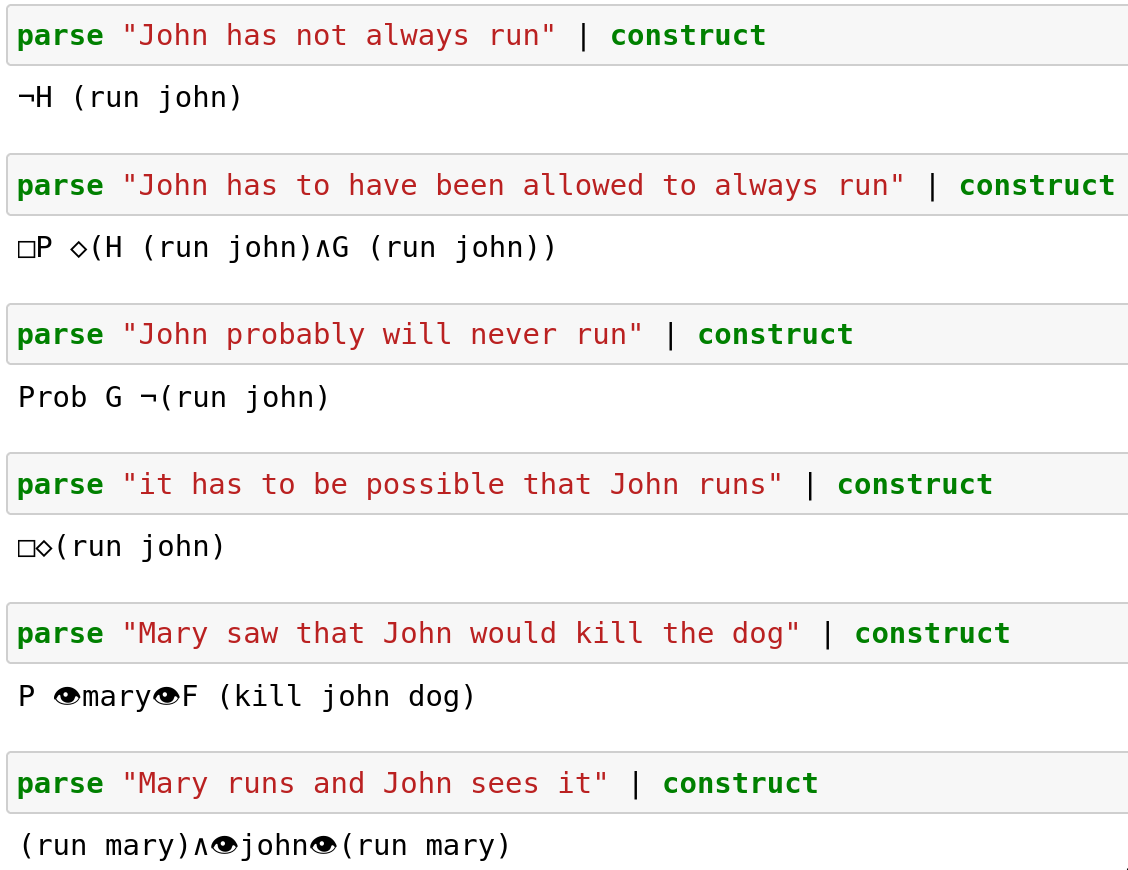
\includegraphics[height=0.85\textheight]{img/glif-intensional.png}
    }
\end{frame}}{}

\ifpart{sometimesnarrow}{\switchtowide}{}

\ifpart{forthelexample}{
\begin{frame}
    \frametitle{Example: ForTheL}
    \autowidth{
        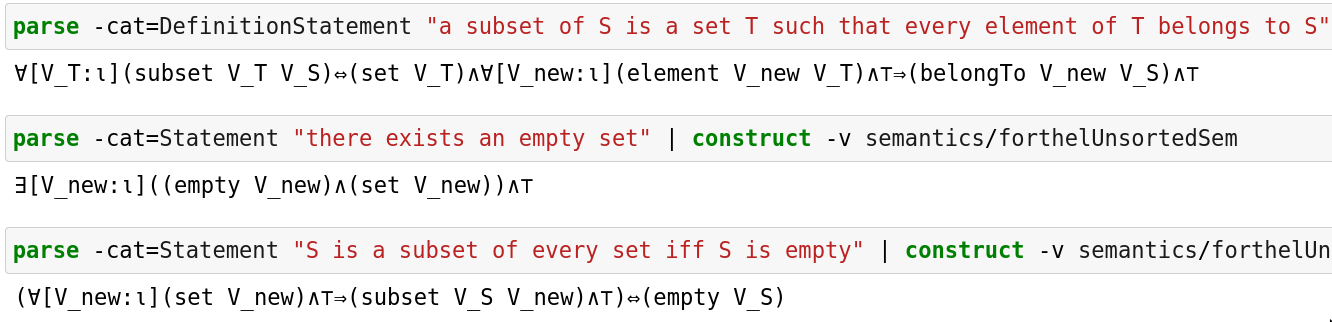
\includegraphics[width=\textwidth]{img/screenshot-glif-forthel.png}
    }
\end{frame}}{}

\begin{frame}
    \frametitle{Components of GLIF: ELPI}
    \enablepart{hlelpi}
    \autowidth{
    \includestandalone[width=\textwidth]{fig/glif-architecture}
    }
\end{frame}

\begin{frame}[fragile]
    \frametitle{Components of GLIF: ELPI}
    \autowidth{
    \begin{itemize}
        \item Implementation and extension of $\lambda$Prolog\com{$\approx$ Prolog + HOAS}
        \item MMT can generate logic signatures
        \ifpart{mentionprovergen}{
            \item First experiments with prover generation
        }{}
        \item Generic inference/reasoning step after semantics construction
        \ifpart{showspa}{\item Goal: Use it for semantic/pragmatic analysis}{}
    \end{itemize}
    \lstset{basicstyle=\footnotesize\ttfamily}

    \vspace{1em}
    \centering
    % Used in slides/glif-components.tex
% Has to be in separate file...
\begin{minipage}[t]{0.35\textwidth}
    \parbox[t][1em][t]{\textwidth}{\centering\bf MMT}\par
    \begin{lstlisting}[language=MMT,linewidth=\textwidth]
o : type //propositions
\neg : o \raa o
\wedge : o \raa o \raa o
\vee : o \raa o \raa o

\iota : type //individuals
\forall : (\iota \raa o) \raa o
\exists : (\iota \raa o) \raa o \end{lstlisting}
\end{minipage}\hskip2em
\begin{minipage}[t]{0.35\textwidth}
    \parbox[t][1em][t]{\textwidth}{\centering\bf ELPI}\par
    \begin{lstlisting}[language=ELPI,linewidth=\textwidth]
kind o type.
not : o -> o.
and : o -> o -> o.
or  : o -> o -> o.

kind i type.
type forall (i -> o) -> o.
type exists (i -> o) -> o.  \end{lstlisting}
\end{minipage}

    \par
%     \begin{minipage}[t]{\textwidth}
%         \centering
%         \begin{minipage}[t]{0.5\textwidth}
%             \begin{lstlisting}[language=ELPI,frame=single]
% kind o type.
% type not o -> o.
% type and o -> o -> o.
% 
% kind i type.
% type forall (i -> o) -> o.
%             \end{lstlisting}
%         \end{minipage}
%     \end{minipage}
    }
\end{frame}

\ifpart{showepistemicexample}{
    \begin{frame}[fragile]
    \def\mybox#1{\square_{#1}}
    \def\mydia#1{\lozenge_{#1}}
    \def\sfiven{{S5_n}}
    \frametitle{Example: Epistemic Q\&A}
    \centering
    \strplain{\makebox[9.5cm][l]{John knows that Mary or Eve knows that Ping has a dog.}\makebox[1.5em]{\upshape($S_1$)}\\
              \makebox[9.5cm][l]{Mary doesn't know if Ping has a dog.}\makebox[1.5em]{\upshape($S_2$)}\\
              \makebox[9.5cm][l]{Does Eve know if Ping has a dog?}\makebox[1.5em]{\upshape($Q$)}}

    {\color{logicfont}
        \begin{align*}
            S_1 &= \mybox{john}(\mybox{mary} hd(ping)\vee \mybox{eve}hd(ping))\\
            S_2 &= \neg(\mybox{mary}hd(ping) \vee \mybox{mary}\neg hd(ping))\\
            Q &= \mybox{eve}hd(ping) \vee \mybox{eve}\neg hd(ping)
        \end{align*}
    }

    \begin{table}
        \begin{tabular}{l l}
            $S_1, S_2 \vdash_\sfiven Q$\quad      &$\leadsto$\quad yes\\
            $S_1, S_2 \vdash_\sfiven \neg Q$\quad &$\leadsto$\quad no\\
            else &$\leadsto$\quad maybe
        \end{tabular}
    \end{table}
\end{frame}

}{}

\ifpart{showspa}{
    \begin{frame}
        \frametitle{Semantic/Pragmatic Analysis}
        \autowidth{
        {
            \centering
            \str{The trophy doesn't fit in the brown suitcase because it's too big.}~\cite{levesque2012winograd}\par
            \pause
            \str{The trophy doesn't fit in the brown suitcase because it's too small.}~\cite{levesque2012winograd}\par
            \pause
            \vspace{1.5em}
            \str{The ball has a radius of $2m$.}\par
            \str{The ball has a mass of $2m$.}\par
            \vspace{1.5em}
            \str{We saw her duck.}\par
        }
        \vspace{2em}
        $\leadsto$ semantics construction creates preliminary semantic representation(s)
        that get refined by the semantic/pragmatic analysis
        }
    \end{frame}
}{}


\ifpart{showjupyter}{
\begin{frame}
    \frametitle{Components of GLIF: Jupyter}
    \enablepart{hljupyter}
    \includestandalone[width=\textwidth]{fig/glif-architecture}
\end{frame}

\begin{frame}
    \frametitle{Components of GLIF: Jupyter}
    \begin{itemize}
        \item Unified, notebook-based interface
        \item Supports implementation and testing
        \item Useful for prototype, demos, teaching, \dots
    \end{itemize}

    \centering
    \vspace{1.5em}
    \fbox{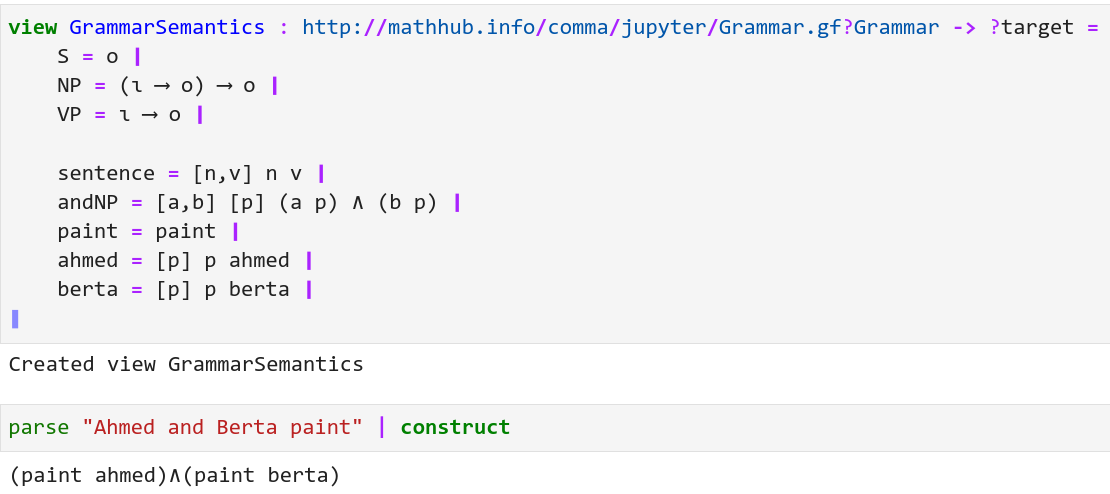
\includegraphics[trim={0 0 20cm 5.7cm},clip,width=0.7\textwidth]{img/screenshot-glif-1.png}}
\end{frame}
}{}
